\SetPicSubDir{ch-Noodle}
\SetExpSubDir{ch-Noodle}

\chapter{Result and Evaluation}
\label{ch:noodle}
\vspace{2em}

\section{Preliminary}
In this chapter, experiments are conducted and performances are evaluated upon the proposed model. We analyze and compare the result of each experiment using a pre-defined metric evaluation. The setup of the experiment is presented in Section 5.2. The results of experiments are presented in Section 5.3, 5.4, and 5.5 where 3 experiments are conducted. Lastly in Section 5.6 we compare 2 different ways of generating a prediction of the selected model.

\section{Experiment}
We investigate different factors that potentially affect the performance of the prediction model, including several window size and response size. We also analyze the evaluation metrics using two interpolation techniques; Spline and Linear interpolation. All development and testing stage are performed via Jupyter Notebook and PyCharm IDE on MacBook-Pro 2.9GHz Dual-Core Intel Core i5, 8GB of RAM, and Intel Iris Graphics 550,  while the model training of 1-month AIS dataset is run on Desktop PC with AMD Ryzen 7 1700 3.0 GHz Eight-Core AM4 processor, 64GB of RAM and GeForce GTX 1080 Ti GPU. We use the following libraries and framework in Python during the course of development; Tensorflow 2.0 for training LSTM model, Scikit-learn for data pre-processing and linear regression modeling, Geopandas for transforming longitude and latitude value into a single coordinate object, Movingpandas for the trajectory analysis and visualization, Kepler.gl for geospatial analytic visualization on the web application, Scipy for variable interpolation, and finally Pandas for data analysis and manipulation. Our final datasets are split into 60\% of training, 20\% of validation, and 20\% of the testing set which translates into 1505106, 501702, and 501702 total datasets respectively. The input-output pair of datasets are generated using a slice generator of tensorflow with shuffling.

We experiment with single-step and multi-step prediction time given a variety of window sizes. Multi-step prediction includes 10 and 30 timesteps in the future. There are two strategies to perform multi-step prediction in AIS time series dataset; (i) direct multi-step and (ii) recursive multi-step. The first part of the experiment uses direct multi-step strategy, and the second part uses recursive multi-step. Direct multi-step involves several models to predict each time step, which means to predict 10 time-step into the future we need to create 10 models; one model for each prediction step. Recursive multi-step in contrary involves only one model being used multiple times where the prior timestep is used as the input for the next prediction, which means to predict 30 timesteps we can either use 10 timestep model for 3 times or single timestep model for 30 times. During the experiment, a model training might stop in a different number of epochs depending on whether the error has reached the limit of early stopping criteria, which is set to 0.0001 deltas for 5 consecutive epochs. Early stopping is a technique introduced in tensorflow to prevent overfitting by stopping the training process when the loss does not improve for multiple stages of training or epochs.

\section{Prediction Model Using 1 Timestep}
We begin our experiment with 1 timestep prediction given several window size of ship movement from 1 to 30 timestep. Our input and target dataset for each sequence are shaped into $\emph{W}\times2$ and $1\times2$ where \emph{W} represents a different value of window size and 1 represent the prediction timestep over 2 features. The input and target shape is applied to training, validation, and testing datasets.

Using Linear interpolation and a window size of 30, our model performance results in 0.0049 MAE and 0.0056 RMSE which translates to the lowest MAPE of 3.50\% over 9 epochs. Lowering the window size to 20, 10 and 1 increase the error of the model as seen in Table 5.1. Compared to other window sizes, a window size of 1 suggests the highest error of 0.0101 MAE. The reason is that neural network does not have enough information to learn the vessel's movement pattern with just one value of observation. The experiment result with Spline interpolation is showing a different trend. Using a window size of 30 the error starts with 0.0049 MAE and 0.0057 RMSE, then go up slightly to 0.0053 MAE and 0.0059 RMSE on the window size of 20, decrease again to 0.0043 MAE and 0.0048 RMSE on the window size of 10, before another increase to 0.0115 MAE and 0.0128 RMSE on the window size of 1. 

\begin{table}[]
\centering
\caption{Model performance with dynamic window size and 1 prediction timestep}
\label{tab:target1}
\resizebox{\textwidth}{!}{%
\begin{tabular}{|c|c|c|c|c|c|c|c|c|}
\multirow{2}{*}{\textbf{Window Size}} &
  \multicolumn{2}{c|}{\textbf{MAE}} &
  \multicolumn{2}{c|}{\textbf{RMSE}} &
  \multicolumn{2}{c|}{\textbf{MAPE (\%)}} &
  \multicolumn{2}{c|}{\textbf{Epochs}} \\ \cline{2-9}
 &
  \textbf{Linear} &
  \textbf{Spline} &
  \textbf{Linear} &
  \textbf{Spline} &
  \textbf{Linear} &
  \textbf{Spline} &
  \textbf{Linear} &
  \textbf{Spline} \\
  \hline
30 & 0.0049 & 0.0049 & 0.0056 & 0.0057 & 3.50 & 3.42 & 9 & 12 \\
20 & 0.0047 & 0.0053 & 0.0053 & 0.0059 & 3.57 & 7.34 & 18 & 10\\
10 & 0.0063 & 0.0043 & 0.0070 & 0.0048 & 4.37 & 3.71 & 9 & 13\\
1 & 0.0101 & 0.0115 & 0.0112 & 0.0128 & 8.53 & 12.32 & 7 & 10\\
\end{tabular}%
}
\end{table}

Figure 4.3 illustrate the plot between the observation (blue), prediction (green), and actual target (red) for 1 minute ahead. Although the error of predicting one timestep into the future is low, it might not be useful in practice. Therefore in the last experiment of section 5.6, we generate bigger prediction timestep recursively using single-step prediction model.

\begin{figure}[b!]
    \centering
    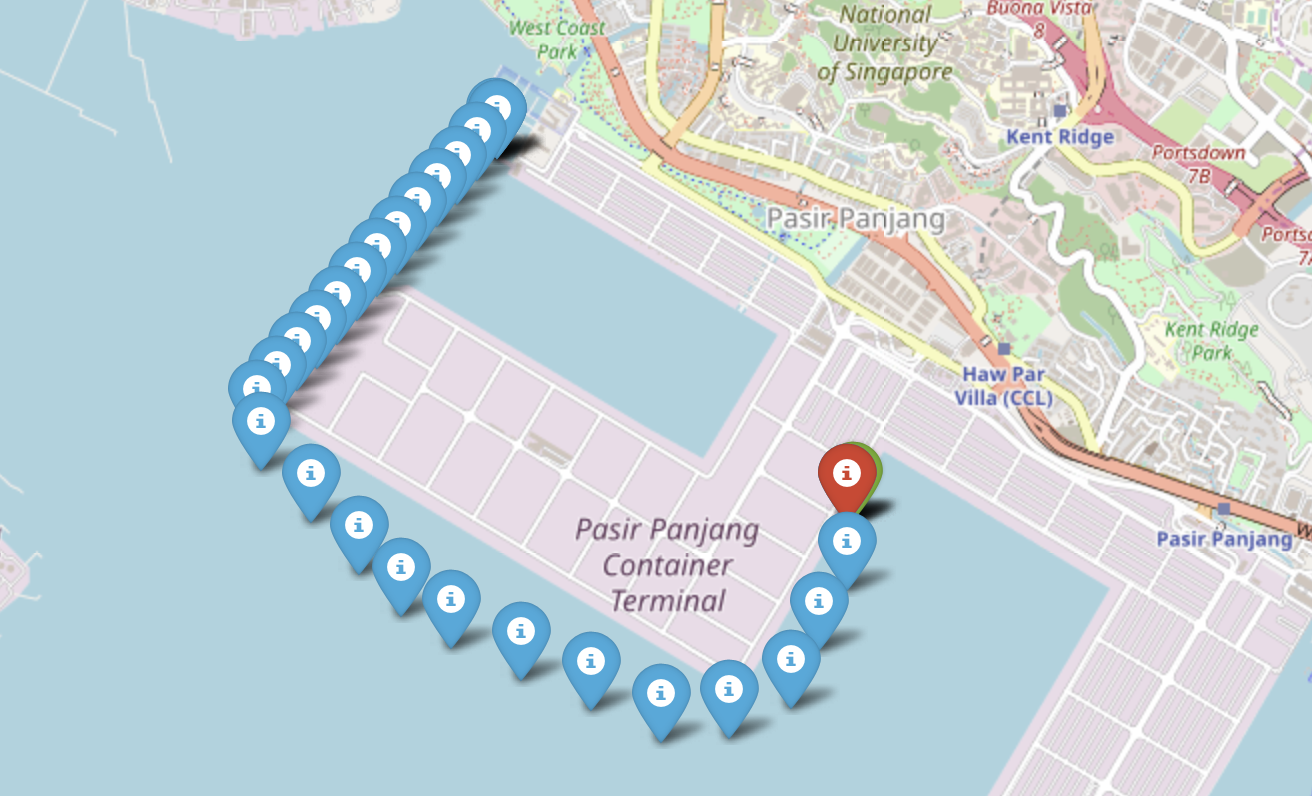
\includegraphics[width=12cm]{pic/ch-Noodle/predictions.png}
    \caption{Plot of 1 timestep prediction given window size of 30}
    \label{fig:predict1}
\end{figure}

\section{Prediction Model Using 10 Timestep}
In this experiment, we develop a model with 10 prediction timestep given a variety of window size. Following the previous experiment, the shape of input and target is $\emph{W}\times2$ and $10\times2$ where \emph{W} indicate the various value of window size and 10 indicate prediction timestep over 2 features of longitude and latitude. The input and target shape is applied to training, validation, and testing datasets.

Using linear interpolation and a window size of 1, the error of the model is 0.0463 MAE, 0.0593 RMSE and 41\% MAPE, the highest error among other window sizes. Once we increase the window size into 10 we see a significant drop in the error with 0.0233 MAE, 0.0332 RMSE and 19\% MAPE. As we further increases the window size by 10 up to 40, the error slightly increase to 0.0238 MAE, 0.0339 RMSE and 20\% MAPE as seen in Table 5.2. The result also suggests that increasing window size to 60 and 80 helps to decrease the error relatively small in MAE, RMSE, and MAPE as compared to the window size of 40.

With spline interpolation, the result suggests a different performance. Other than window size of 1, the MAE has an upward trend as the window size goes up until 80. Table 5.2 clarifies this point. It starts at 0.0169 MAE and 1.0240 RMSE on the window size of 10 and 20 and continuously goes up until 0.0195 MAE and 0.0269 RMSE on the last window size. The MAPE metrics on spline does not correlate proportionally with MAE despite MAPE is a percentage form of MAE. On window size of 10 and 20, while the MAE share the same error, the MAPE differ very significantly by 29\% and 103\% respectively. On window size of 30, the MAE increase from the previous window size while the MAPE however decrease. The highest MAE and the lowest MAPE come from the same window size of 80. 

The trend of MAPE with spline interpolation might indicate that MAPE as a performance metric, in general, has a pitfall for some reasons. First, MAPE would fail if some of the actual values are zero. Second, MAPE would result in extremely high number if some of the actual values are very close to zero and therefore bias the informativeness of MAPE \cite{hyndman2006another}. The issue could happen to any dataset, including AIS time series, being standardized using mean and standard deviation as the transformation would be centred in 0 points. We shall take the information from MAPE metrics with a grain of salt and use MAE and RMSE for cross-validation.

\begin{table}[t!]
\centering
\caption{Model performance with dynamic window size and 10 prediction timestep}
\label{tab:target10}
\resizebox{\textwidth}{!}{%
\begin{tabular}{|c|c|c|c|c|c|c|c|c|}
\multirow{2}{*}{\textbf{Window Size}} &
  \multicolumn{2}{c|}{\textbf{MAE}} &
  \multicolumn{2}{c|}{\textbf{RMSE}} &
  \multicolumn{2}{c|}{\textbf{MAPE (\%)}} &
  \multicolumn{2}{c|}{\textbf{Epochs}} \\ \cline{2-9}
 &
  \textbf{Linear} &
  \textbf{Spline} &
  \textbf{Linear} &
  \textbf{Spline} &
  \textbf{Linear} &
  \textbf{Spline} &
  \textbf{Linear} &
  \textbf{Spline} \\
  \hline
80 & 0.0225 & 0.0195 & 0.0320 & 0.0269 & 19.39 & 14.02 & 35 & 24 \\
60 & 0.0229 & 0.0172 & 0.0326 & 0.0242 & 19.97 & 77.22 & 32 & 42 \\
40 & 0.0238 & 0.0173 & 0.0339 & 0.0242 & 20.04 & 58.59 & 27 & 34 \\
30 & 0.0239 & 0.0181 & 0.0340 & 0.0256 & 20.05 & 87.57 & 27 & 34 \\
20 & 0.0234 & 0.0169 & 0.0333 & 0.0240 & 19.68 & 103.08 & 27 & 50\\
10 & 0.0232 & 0.0170 & 0.0332 & 0.0240 & 19.10 & 29.46 & 36 & 50\\
1 & 0.0463 & 0.0590 & 0.0593 & 0.0744 & 41.15 & 70.47 & 50 & 14\\
\end{tabular}%
}
\end{table}

\begin{figure}[t!]
\centering
\begin{subfigure}[b]{0.45\textwidth}
  \centering
  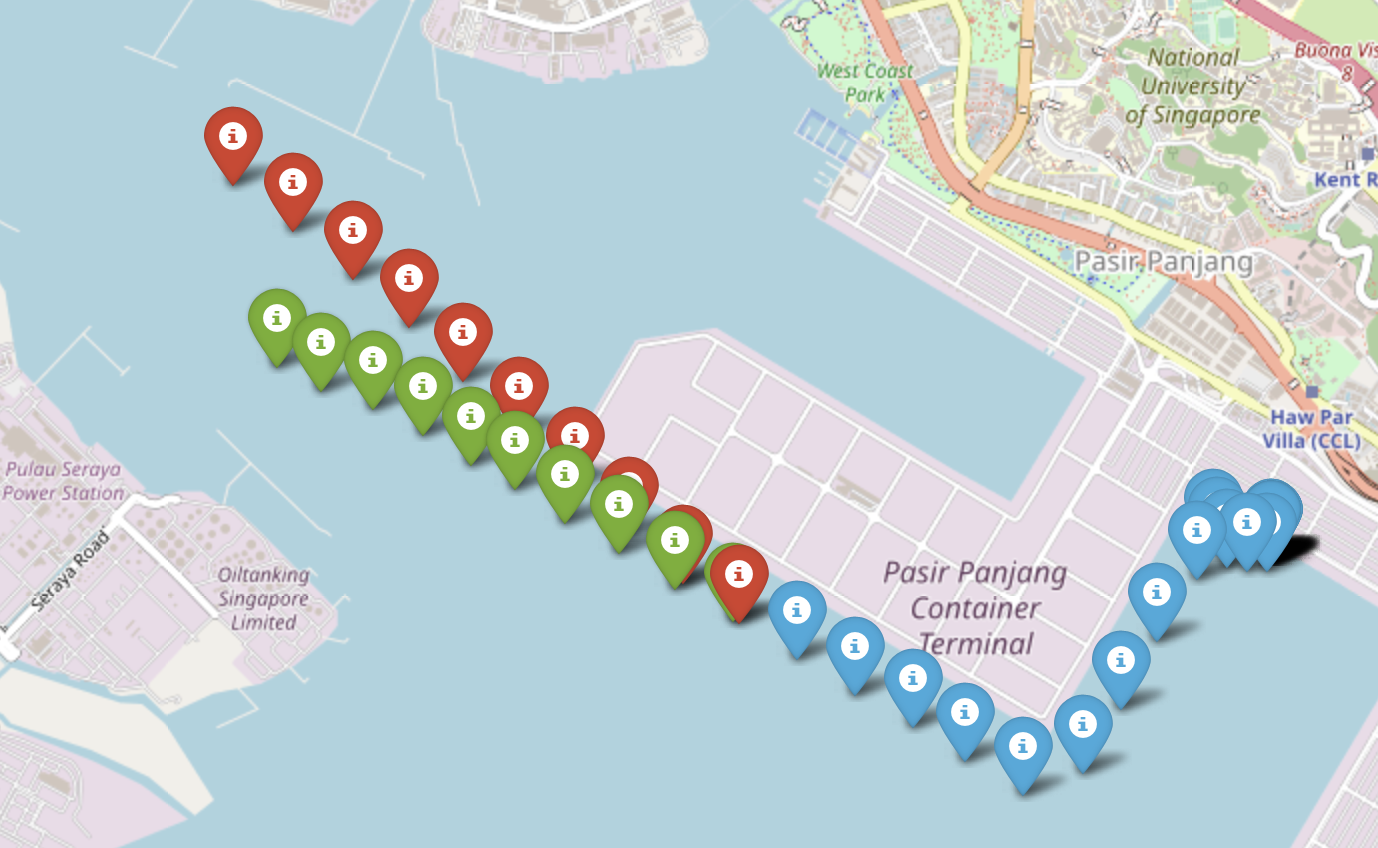
\includegraphics[width=1\linewidth]{pic/ch-Noodle/predict3010.png}
  \caption{Plot of 10 timestep prediction given window size of 30}
  \label{fig:predict3010}
\end{subfigure}
%
\begin{subfigure}[b]{0.5\textwidth}
  \centering
  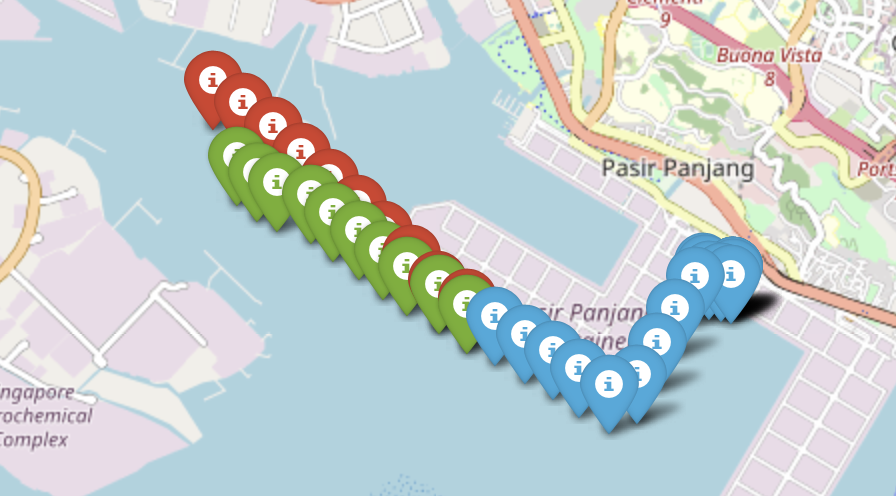
\includegraphics[width=1\linewidth]{pic/ch-Noodle/predict3010_3.png}
  \caption{Plot of 10 timestep prediction given window size of 20}
  \label{fig:predict2010}
\end{subfigure}
\caption{Plot of 10 timestep prediction}
\label{fig:predict10}
\end{figure}

Predicting the vessel's position for the next 10 timesteps is certainly more useful in practice than just 1 timestep. To help us better visualize the model performance, we plot a certain ship track from the prediction model using linear interpolation. The blue, red, and green colour in Figure 5.2 represents observation, actual target, and prediction respectively. Figure 5.2 shows a trajectory with 10 timestep prediction and the window size of 30 and 20. Figure 5.2b shows more accurate prediction as compared to 5.2a.

\section{Prediction Model Using 30 Timestep}
Lastly, we experiment with 30 prediction timestep given a variety of window size. Our input and target dataset for each sequence are shaped into $\emph{W}\times2$ and $30\times2$ where \emph{W} represents a different value of window size and 30 represent the prediction timestep over 2 features, longitude and latitude. This input and target shape is applied to training, validation, and testing datasets.

\begin{table}[t!]
\centering
\caption{Model performance with dynamic window size and 30 prediction timestep}
\label{tab:target10}
\resizebox{\textwidth}{!}{%
\begin{tabular}{|c|c|c|c|c|c|c|c|c|}
\multirow{2}{*}{\textbf{Window Size}} &
  \multicolumn{2}{c|}{\textbf{MAE}} &
  \multicolumn{2}{c|}{\textbf{RMSE}} &
  \multicolumn{2}{c|}{\textbf{MAPE (\%)}} &
  \multicolumn{2}{c|}{\textbf{Epochs}} \\ \cline{2-9}
 &
  \textbf{Linear} &
  \textbf{Spline} &
  \textbf{Linear} &
  \textbf{Spline} &
  \textbf{Linear} &
  \textbf{Spline} &
  \textbf{Linear} &
  \textbf{Spline} \\
  \hline
80 & 0.0697 & 0.0751 & 0.0981 & 0.1053 & 63.96 & 70.29 & 35 & 45 \\
60 & 0.0746 & 0.0782 & 0.1041 & 0.1098 & 68.41 & 73.61 & 25 & 37 \\
40 & 0.0744 & 0.0772 & 0.1044 & 0.1081 & 67.70 & 70.54 & 21 & 50 \\
30 & 0.0762 & 0.0770 & 0.1070 & 0.1080 & 67.96 & 71.18 & 26 & 50 \\
20 & 0.0772 & 0.0784 & 0.1082 & 0.1098 & 68.88 & 72.30 & 26 & 50\\
10 & 0.0840 & 0.0803 & 0.1182 & 0.1125 & 71.75 & 73.09 & 22 & 50\\
1 & 0.1426 & 0.1346 & 0.1790 & 0.1701 & 114.26 & 108.97 & 13 & 22\\
\end{tabular}%
}
\end{table}

\begin{figure}[b!]
    \centering
    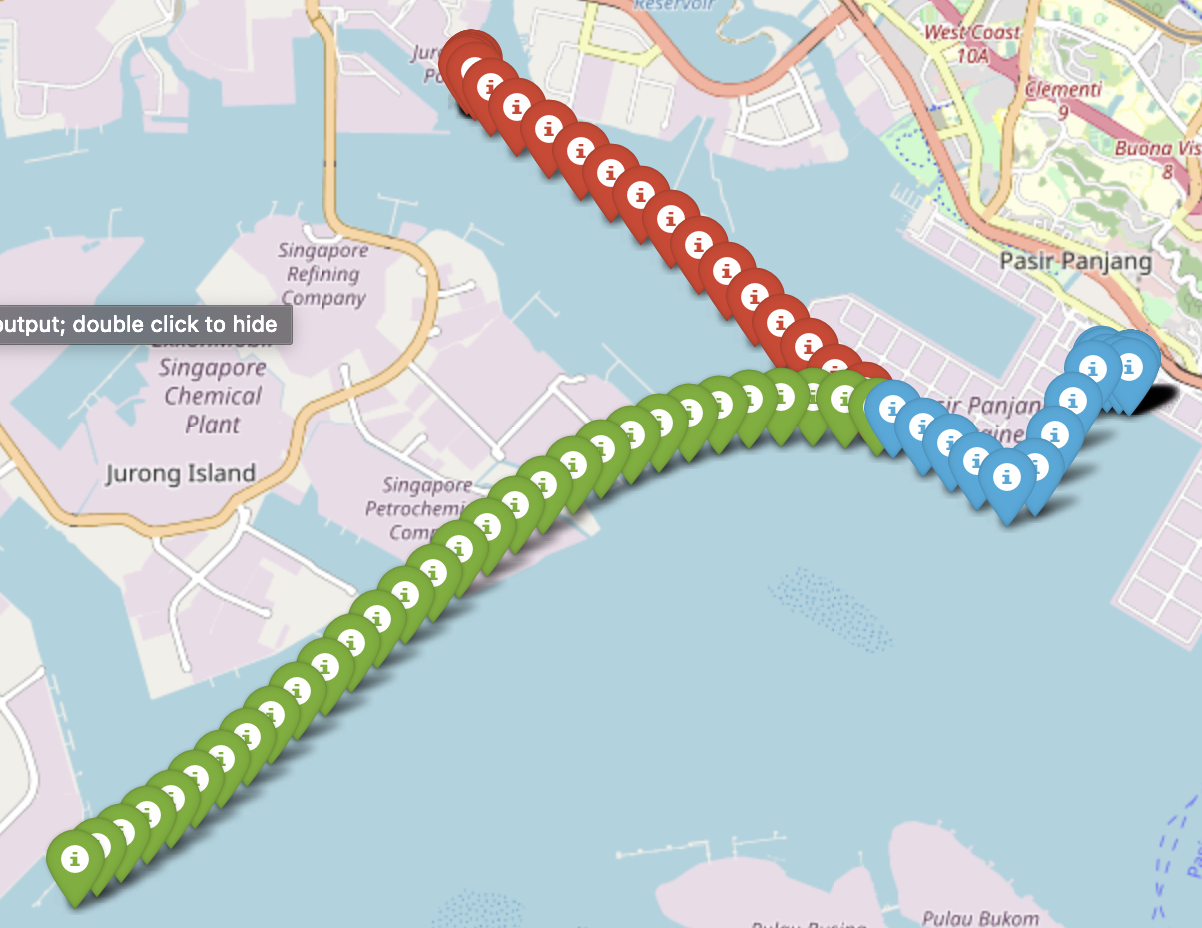
\includegraphics[width=8cm]{pic/ch-Noodle/predict3030.png}
    \caption{Plot of 30 timestep prediction using window size of 30}
    \label{fig:predict3030_1}
\end{figure}

\begin{figure}[t!]
\centering
\begin{subfigure}[b]{.30\textwidth}
  \centering
  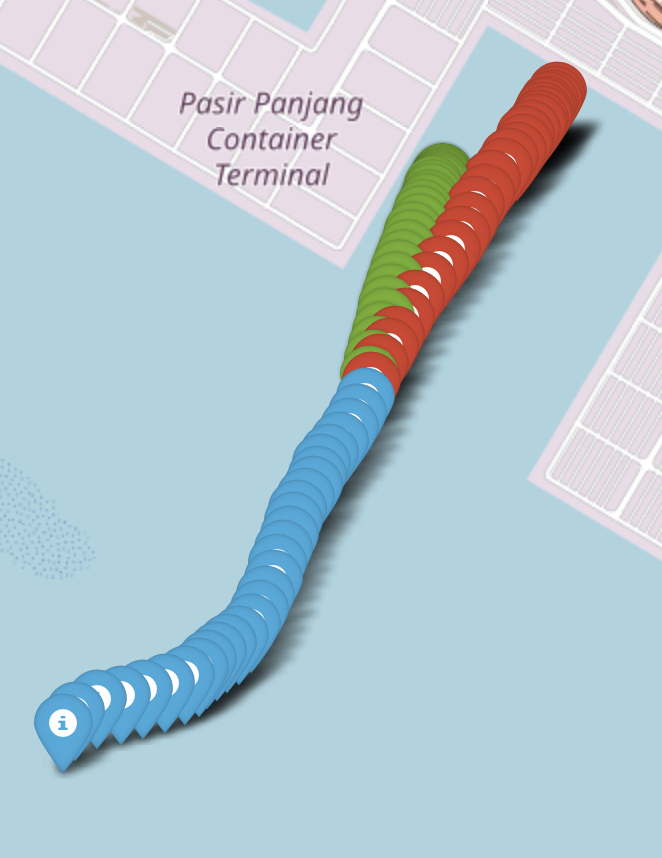
\includegraphics[width=1\linewidth]{pic/ch-Noodle/predict3030_2.png}
  \caption{Plot of 30 timestep prediction for straight past trajectory}
  \label{fig:predict3030_2}
\end{subfigure}
%
\begin{subfigure}[b]{.33\textwidth}
  \centering
  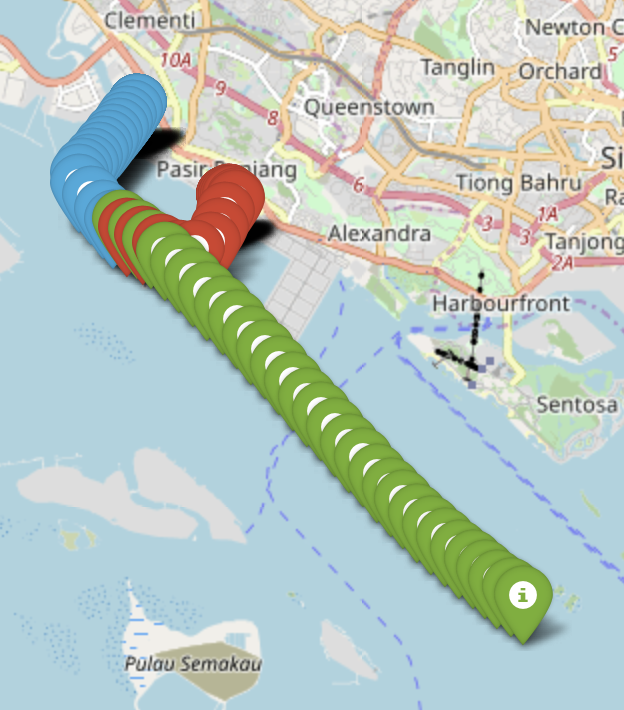
\includegraphics[width=1\linewidth]{pic/ch-Noodle/predicted3030_4.png}
  \caption{Plot of 30 timstep prediction for non-straight past trajectory}
  \label{fig:predict3030_3}
\end{subfigure}
\caption{Plot of 30 timestep prediction with window size of 30}
\label{fig:predict3030}
\end{figure}

With linear interpolation, beside the window size of 1, the error of the model decrease from 0.0840 MAE, 0.1182 RMSE and 71.75\% MAPE to 0.0697 MAE, 0.0981 RMSE, and 63.96\% MAPE as we increase the window size from 10 to 80 as seen in Table 5.3. With spline interpolation, the performance metrics indicate the same trend as the one in linear interpolation. Beside window size of 1, the error starts at 0.0803 MAE, 0.1125 RMSE, and 73\% MAPE on the window size of 10, and progressively decrease to 0.0751 MAE, 0.1053 RMSE, and 70.29\% MAPE on window size 80. Looking at the MAPE, all window size in this experiment are categorized as an inaccurate model.

We can see from the plot in Figure 5.4a and Figure 5.4b, with window size 30, the predicted trajectory suffer from big deviation when the past trajectory tends to be non-straight. In contrary, the prediction is more accurate when the past trajectory is straight. We plot the same track on window size 40 which overall has lower error than window size 30. Having longer window size help reduce the error as the predicted track tend to be closer to the actual track as seen in Figure 5.5.

\begin{figure}[t!]
    \centering
    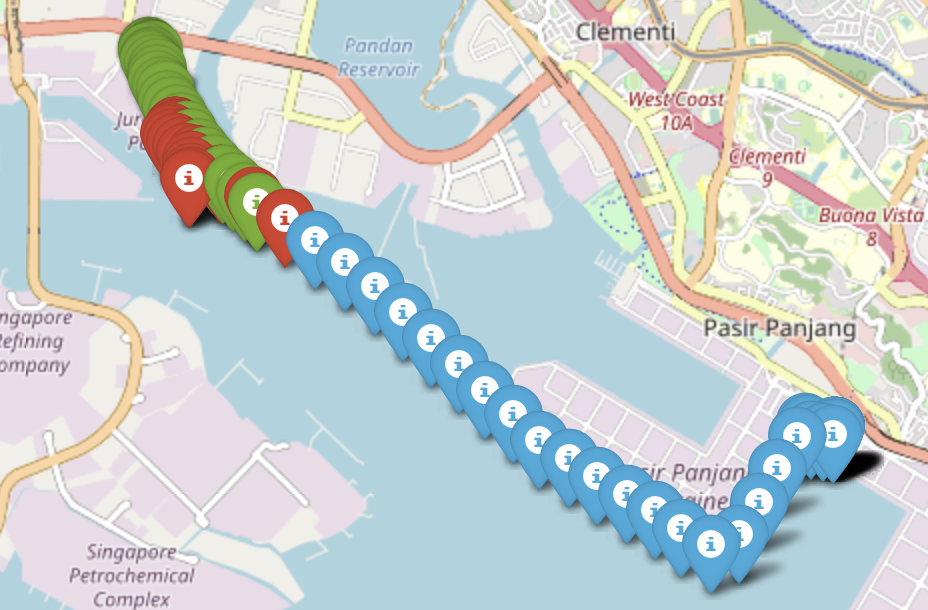
\includegraphics[width=8cm]{pic/ch-Noodle/predict3040.png}
    \caption{Plot of 30 timetep prediction using window size of 40}
    \label{fig:predict3030_1}
\end{figure}

\section{Recursive Multi-step Prediction}
Recall that recursive multi-step prediction makes use of the same model to generate multiple predictions recursively, meaning the output from the previous timestep become the input in the next prediction. In this experiment, we generate 30 timestep prediction with 3 methods, (i) direct prediction with 30 timesteps, (ii) recursive prediction with 10 timestep model for 3 times, (iii) recursive prediction with 1 timestep model for 30 times. The first method is the one we see in section 5.5 and Figure 5.3. To allow comparable result we pick one model in previous experiments from the same window size, evaluate the performance metrics and plot the track for visualization. 

\begin{figure}[t!]
\centering
\begin{subfigure}[b]{.45\textwidth}
  \centering
  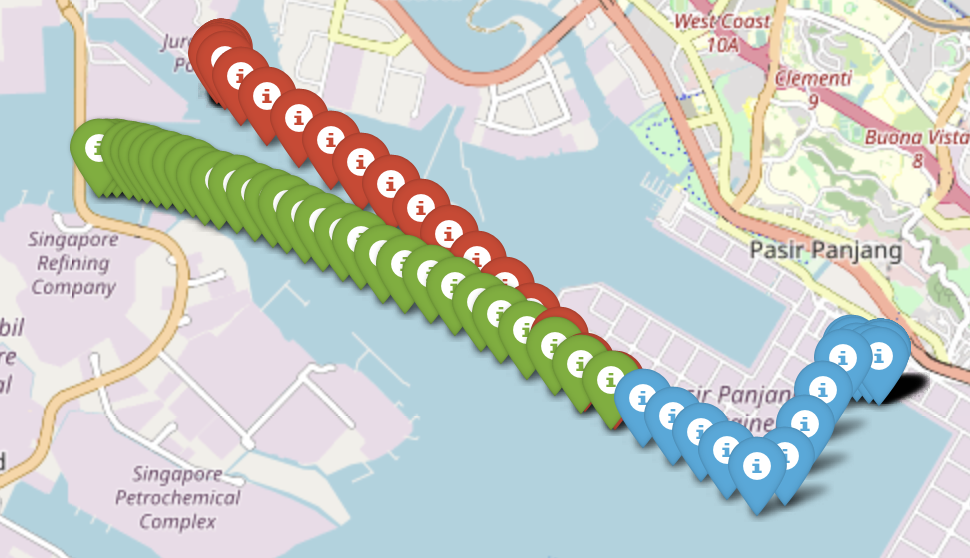
\includegraphics[width=1\linewidth]{pic/ch-Noodle/recursive30_from10.png}
  \caption{Plot of 30 timestep prediction using 10 timestep model}
  \label{fig:recursive30_10}
\end{subfigure}
%
\begin{subfigure}[b]{.47\textwidth}
  \centering
  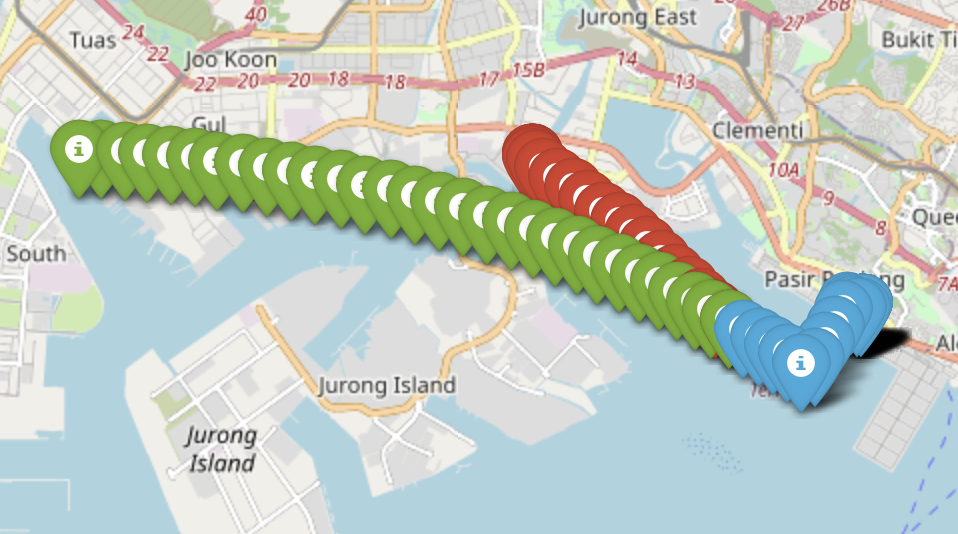
\includegraphics[width=1\linewidth]{pic/ch-Noodle/recursive30_from1.png}
  \caption{Plot of 30 timestep prediction using 1 timestep model}
  \label{fig:recursive30_1}
\end{subfigure}
\caption{Plot of 30 timestep prediction using window size of 30}
\label{fig:recursive30}
\end{figure}

\begin{figure}[t!]
\centering
\begin{subfigure}[b]{.45\textwidth}
  \centering
  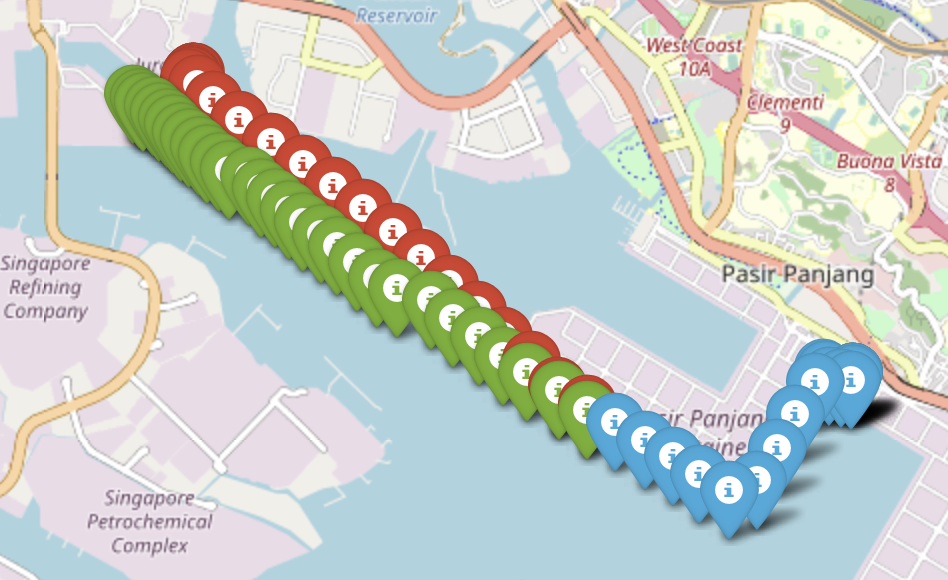
\includegraphics[width=1\linewidth]{pic/ch-Noodle/recursive20_from10.png}
  \caption{Plot of 30 timestep prediction using 10 timestep model}
  \label{fig:recursive20_10}
\end{subfigure}
%
\begin{subfigure}[b]{.47\textwidth}
  \centering
  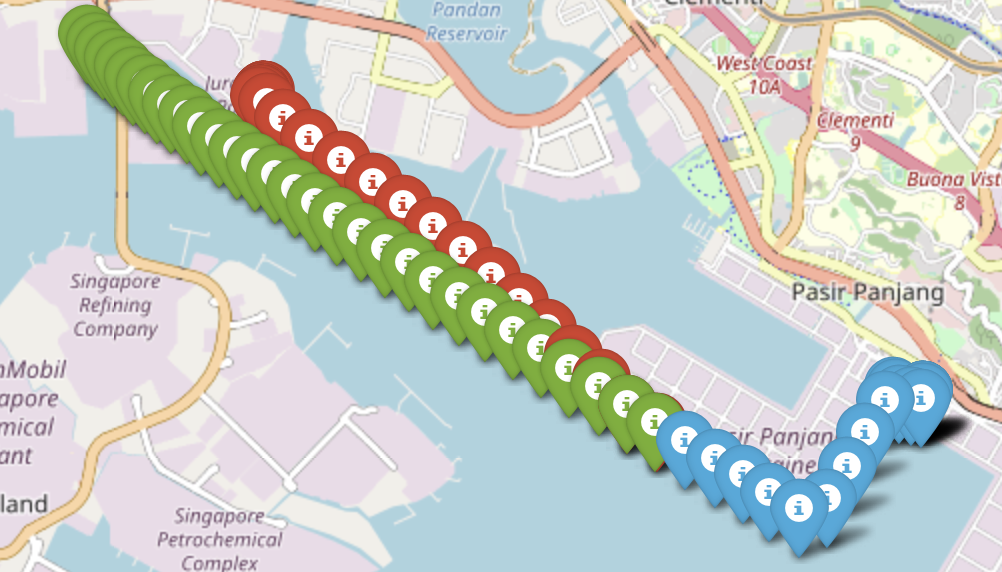
\includegraphics[width=1\linewidth]{pic/ch-Noodle/recursive20_from1.png}
  \caption{Plot of 30 timestep prediction using 1 timestep model}
  \label{fig:recursive20_1}
\end{subfigure}
\caption{Plot of 30 timestep prediction using window size of 20}
\label{fig:recursive20}
\end{figure}

\begin{figure}[t!]
\centering
\begin{subfigure}[b]{.45\textwidth}
  \centering
  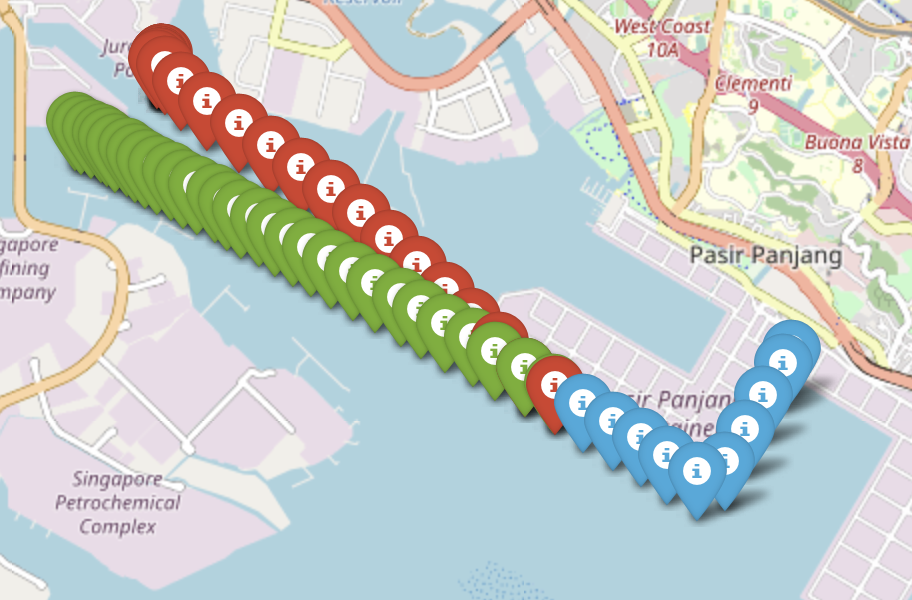
\includegraphics[width=1\linewidth]{pic/ch-Noodle/recursive10_from10.png}
  \caption{Plot of 30 timestep prediction using 10 timestep model}
  \label{fig:recursive10_10}
\end{subfigure}
%
\begin{subfigure}[b]{.48\textwidth}
  \centering
  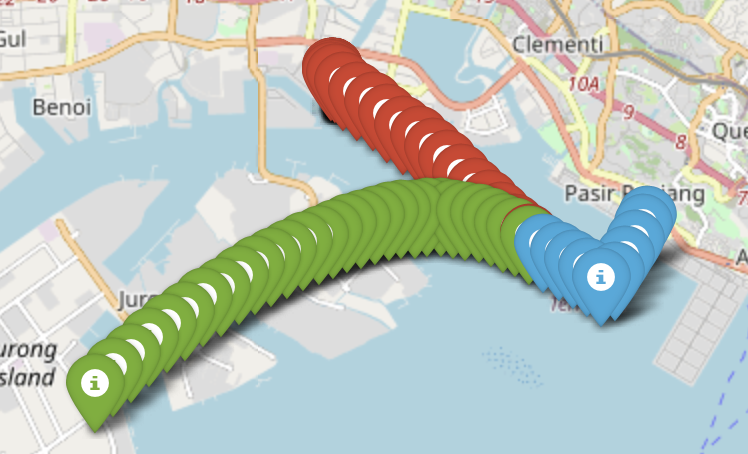
\includegraphics[width=1\linewidth]{pic/ch-Noodle/recursive10_from1.png}
  \caption{Plot of 30 timestep prediction using 1 timestep model}
  \label{fig:recursive10_1}
\end{subfigure}
\caption{Plot 30 timestep prediction recursively using window size of 10}
\label{fig:recursive10}
\end{figure}

Using a window size of 30, the second method suggests a better performance looking at the error scores; 0.0958 MAE, 0.1234 RMSE, and 24.24\% MAPE. The third method did not improve the performance as the error score suggests at 0.2021 MAE, 0.3332 RMSE, and 151.64\% MAPE The plot to validate this result is presented in Figure 5.6.

Using windows size of 20, the second method gives even lower error score compared to the same method on the window size of 30. Its performance metrics results in 0.0628 MAE, 0.0833, and 11.81\% MAPE. The third method's performance metrics score relatively the same as the second method at 0.0619 MAE, 0.0820 RMSE, and 68.33\% MAPE. Figure 5.7 helps us visualize the difference between the two methods.

In the last experiment with a window size of 10, the error in the second method score at 0.0877 MAE, 0.1142 RMSE, and 17.23\% MAPE, slightly higher than the same method on the window size of 20. The performance metrics of the third method is significantly higher as compared to the first method at 0.3033 MAE, 0.4254 RMSE, and 438.38\% MAPE. Figure 5.8 shows the plot between the two methods. We do not experiment with a window size of 1 as the results are known to be poor across all timestep prediction in the previous experiments. 

The result of this experiment suggests that recursive multi-step prediction can effectively improve the performance of long prediction timestep without changing the architecture complexity of neural network model. Specifically, the 10 timestep model with a window size of 20 is proven to have the lowest error metrics as compared to other base models in predicting 30 timesteps.

\section{Summary}
In this chapter, we conducted experiments about the trajectory prediction model using AIS time-series dataset and evaluate the performance with 3 defined metrics, MAE, RMSE, and MAPE. Two interpolation techniques, linear and spline, was used and analysed in each experiment. The first three prediction models categorized as direct multi-step prediction were discussed, including 1, 10, and 30 timesteps with a variation of window size each. The last prediction model is also called recursive multi-step where it recursively generates 30 timestep prediction using 1 and 10 timestep base model. 